\chapter{Conceptos preliminares}
En este capítulo, se presentan algunos conceptos que conviene conocer. En primer lugar, al fenómeno que da pie a este estudio: la Enfermedad del Dragón Amarillo, que no es un tema menor, puesto que se ha extendido por prácticamente todo el mundo y causa pérdidas en los cultivos de cítricos, incluyendo a los cultivos mexicanos. Posteriormente, se hablará sobre los \textit{sistemas dinámicos complejos} para brindar un contexto sobre la doctrina y el enfoque de este trabajo. Este tema fundamenta la relación que existe entre este trabajo y la física. Finalmente, se hablará de la simulación computacional y su relevancia para el desarrollo de este texto, dejando para los capítulos siguientes un resumen de la metodología inicial y los resultados encontrados a través de esta labor\\
En los árboles de las plantaciones de cítricos del campo mexicano, suele habitar un insecto de entre 3 y 4 milímetros \cite{aleman2007diaphorina}; este insecto, llamado \textit{Diaphorina Citri}, es el transmisor de un tipo de bacteria \textit{Liberibacter}, que es la causante del Huanglongbing, que significa «enfermedad del dragón amarillo» en chino, de modo que en este trabajo se hará referencia a ella de ambas formas, así como mediante la abreviatura «HLB».\\
Existe registro de tres variantes distintas de la bacteria que causa el HLB: la variante americana, la asiática y la africana \cite{senasica2017manual}. En México, hay una fuerte presencia de la variante asiática, que es resistente a las altas temperaturas de las regiones tropicales del país. Actualmente, no existe ningún cítrico comercial que sea resistente a esta enfermedad, además de que tampoco existe una cura viable. En las zonas con baja incidencia de esta enfermedad, se previene el esparcimiento de los brotes a través de la remoción de los árboles infectados, de modo que es importante la detección temprana de los contagios, así como una buena estrategia para identificar a los casos asintomáticos. Controlar al vector de transmisión, en este caso el psílido, suele ser la estrategia más común. Hoy día, el HLB ha pasado a ser considerado la enfermedad de cítricos más seria, causando pérdidas de cultivos y árboles desde hace tiempo en Asia y África; y, en los últimos años, en América, dado su rápido crecimiento.\cite{robles2012protocolo}\\
Aunque sus orígenes no están claros, se sabe que esta enfermedad es relativamente nueva en los cítricos, que no alojan de forma natural a esta bacteria, pues no presentan ningún tipo de tolerancia o inmunidad a ella. La primera aparición que se documentó fue en una revista india a principios de la década de 1920, y fue atribuida directamente al psílido, a pesar de que algunas deficiencias nutricionales y problemas en las raíces suelen causar efectos muy parecidos a los del HLB. No obstante, fue hasta una década después que se comenzaron a evaluar las infecciones a través de estudios de laboratorio y no a simple vista, en ese momento comenzó a cobrar relevancia la idea de esta nueva enfermedad en el registro científico formal. El HLB se esparcía rápidamente en China, de dónde saltó a muchos otros países, particularmente los del sureste asiático. La confirmación de su llegada a América se dio con la primera detección en 2005 en Florida, y posteriormente en el Caribe, y en México en 2002.\cite{gottwald2007citrus}\\

%-----------------------------------------------------------Qué es el HLB
\section{La Enfermedad del Dragón Amarillo}
A continuación se describirán algunos aspectos a tener en cuenta sobre el HLB, tales como su historia, sus síntomas y forma de infección, y su importancia económica. En este texto se usará recurrentemente la palabra «asintomático» para referirse a un árbol que es incubador de la bacteria que causa el HLB, pero no parece a simple vista estar contagiado.

\subsection{Historia breve del descubrimiento del HLB}
%Historia
Aunque se ha considerado ampliamente que el HLB se originó en China, la evidencia no parece favorecer esta idea, pues hay indicios de que esto es más bien una confusión histórica, y que quizás el hecho de que fueran los granjeros chinos quienes acuñaran el término «Huanglongbing», propició que los investigadores de otros países asociaran esta enfermedad a este país de forma errónea. Y aunque no está completamente claro por qué se atribuye el HLB a China, hay una certeza razonable de que fueron Husain y Nath en 1927 \cite{chohan2007molecular} los primeros que documentaron los síntomas que observaban en las plantaciones indias, mucho antes de que Hoffman hiciera lo propio para China hasta 1936 \cite{hoffmann1936congenital}. En ambos países, sintomatología similar a la del HLB fue descrita ya desde el siglo XIX \cite{da2010etiology}, sin embargo, dado que puede ser fácilmente confundida con otros problemas, no se puede afirmar que estos síntomas hayan sido causados por el HLB.\\
Naturalmente, esta bacteria -Liberibacter- no surgió en el siglo XIX, sino que debe tener algunos cuantos millones de años de existencia; sin embargo, su aparición en los cultivos de cítricos sí que parece ser reciente, hablando de un par de centenas de años. Esta idea es reforzada por lo débiles que son estos cítricos en contra de este patógeno, pues no parecen estar preparados contra él, a pesar de que los primeros cultivos de cítricos comenzaron alrededor de hace cuatro mil años, un tiempo razonable para que hubiesen ya desarrollado alguna forma de defensa. Finalmente, se ha encontrado que el hábitat natural de esta bacteria son algunas rutáceas africanas.\cite{da2008biology}\\

\subsection{Sintomatología}
%Sintomatología
Dado que algunos de los árboles infectados con HLB suelen ser asintomáticos, los brotes pueden ser difíciles de detectar. Algunos de los árboles que no muestran síntomas pueden tardar incluso años en mostrar los primeros signos de enfermedad. El síntoma más común, y uno de los primeros que suele aparecer, es el característico cambio de color de las hojas que da el nombre de “Dragón Amarillo”, y que está caracterizado por manchas en las hojas son comúnmente asimétricas respecto al nervio principal\cite{mora2012huanglongbing}. Como se ha dicho anteriormente, es posible confundir las deficiencias nutrimentales, incluso para los agricultores más experimentados; el criterio se basa a menudo en la forma de las manchas. Cuando la planta no padece HLB y tiene más bien otro tipo de problema, las manchas amarillas se ven delimitadas por las venas de la hoja y no se vuelven simétricas. Cuando la planta padece HLB,  como las venas son simétricas, el patrón resultante por esta delimitación es también simétrico y con manchas bien definidas. Y aunque este criterio es útil, es más bien un truco del oficio agricultor y carece de rigor científico, de modo que no es suficiente para tener certeza de que algún árbol esté o no contagiado. Este es un problema particular entre los citricultores mexicanos.\\
Otro síntoma es el desprendimiento excesivo de los frutos, que presentan deformidades y decoloración. Este es el síntoma que convierte al HLB en un problema para los citricultores, pues estos frutos con desprendimiento prematuro suelen ser naturalmente más pequeños en promedio que los frutos de un árbol sano, además de que son asimétricos y se caen antes de madurar. Al examinar cualquiera de estos frutos por dentro, se notará que están decolorados y sus semillas están malogradas y oscurecidas \cite{gottwald2007citrus}.  Sería tentador que estos frutos, a pesar de su mala apariencia, alcanzaran el mercado, aunque con un razonable precio menor; pero resulta que no solo su aspecto es malo, también su sabor, carente de dulzura y comúnmente amargo, además de que estos frutos tienen distintos niveles de fructuosa, glucosa y ácido cítrico, de modo que la cosecha de un árbol infectado es casi en su totalidad pérdida. Existen algunos usos que se pueden dar a este tipo de frutas, pero es prácticamente nulo, por lo que un árbol infectado con HLB está condenado a una vida corta e improductiva.\cite{dala2019effect}
A continuación, se muestra una ilustración extraída de la Ficha Técnica del HLB, publicada en 2010 por el Servicio Nacional De Sanidad, Inocuidad y Calidad Agroalimentaria (SENASICA).

\begin{figure}[H]
\centering
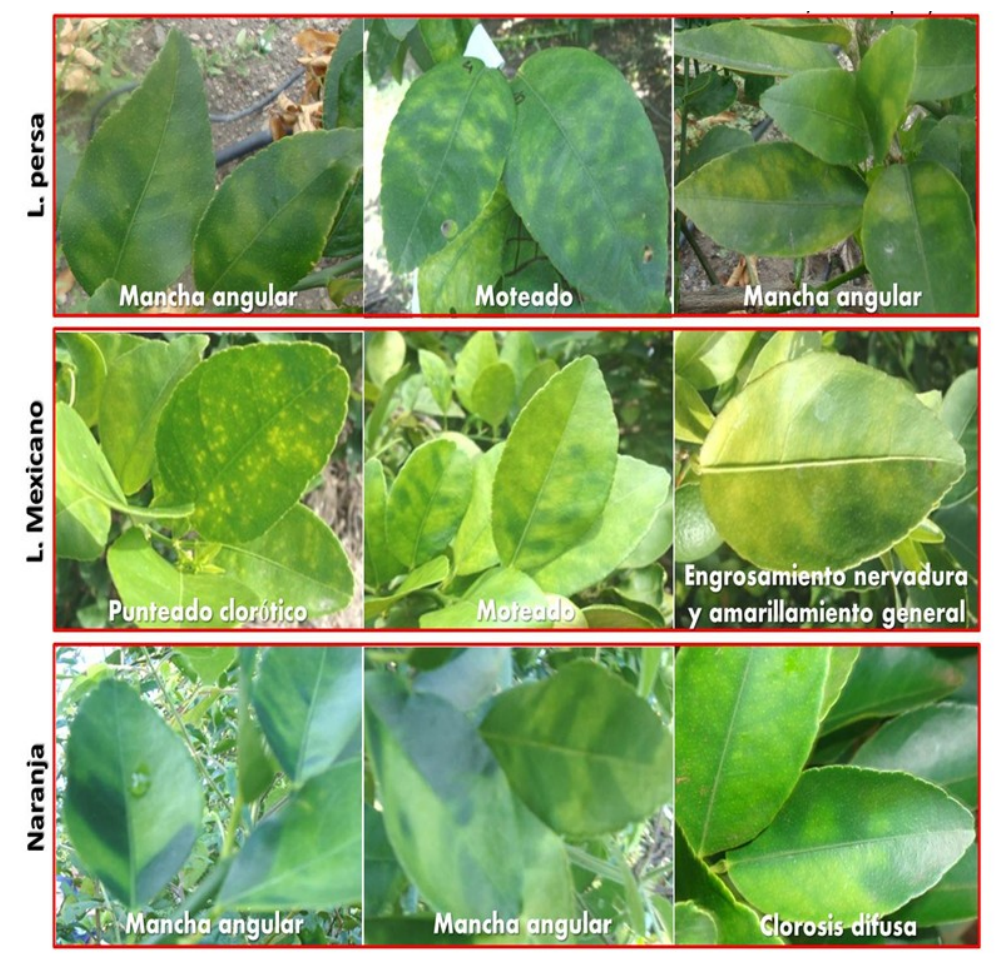
\includegraphics[width=1\textwidth,keepaspectratio=true]{images/C2/1.PNG}
\caption{Síntomas de HLB observados en hojas de limón persa, lima mexicana y naranja dulce, (Fotografía: GIIIC-CP. F. Esquivel y J. Flores, 2010.)}
\end{figure}

\subsection{Modo de transmisión}
%Transmisión y psílidos
Aunque originalmente se pensó que la naturaleza del HLB era viral, posteriormente se tuvo evidencia de que la causa era bacteriana, estas bacterias que se esparcían por los cítricos a través de insectos, estos agentes de transmisión son llamados vectores. Esta infección es diversa y no se limita a algún tipo de clima particular, debido a que a menudo es transmitida por diferentes especies de psílidos que habitan en ambientes diversos. Los cultivos de cítricos que hay en México, tienen las condiciones cálidas y húmedas de las regiones tropicales, de modo que estos cultivos tienen como vector de transmisión al psílido asiático de los cítricos: \textit{Diaphorina citri}, que, como se ha discutido antes, llegó a la región a través de las actividades de la agricultura y es propia de las zonas de siembra.\\

Por otro lado, cuando se observan los cultivos de cítricos en el continente africano, se aprecia que las condiciones son por lo general más frías, y que la bacteria se transmite esta vez por el psílido africano de los cítricos: Trioza erytreae, un insecto intruso al que le favorecen los climas frescos y húmedos y fomentan su crecimiento. Los ejemplares de  Diaphorina Citri nacen de huevecillos que el adulto deposita en los brotes de los árboles, encima y entre los espacios que hay entre las hojas nacientes. Los huevos suelen estar todos concentrados en las mismas ramas de brotes tiernos. Una vez nacen, las ninfas son sedentarias, se establecen sobre estas mismas ramas jóvenes y forman colonias. Para el caso de   Diaphorina citri, se  tiene un periodo embrionario de casi 10 días en un entorno de 15 grados centígrados y de 3.5 días cuando el entorno está a 28 grados centígrados. El tiempo total desde que se deposita el huevo hasta que se convierte en adulto es de aproximadamente 15 días a 28 grados centígrados  y de 49 días a 25 grados centígrados, de modo que las temperaturas entre los 25 y 28 grados centígrados estimulan su desarrollo, sin embargo, un exceso de temperatura tampoco es favorable, pues el psílido no es capaz de desarrollarse en temperaturas que excedan los 33 grados centígrados, teniendo a su vez como cota inferior los diez grados centígrados. A continuación, se muestra una ilustración extraída de la Ficha Técnica del HLB y publicada en 2010 por el SENASICA.

\begin{figure}[H]
\centering
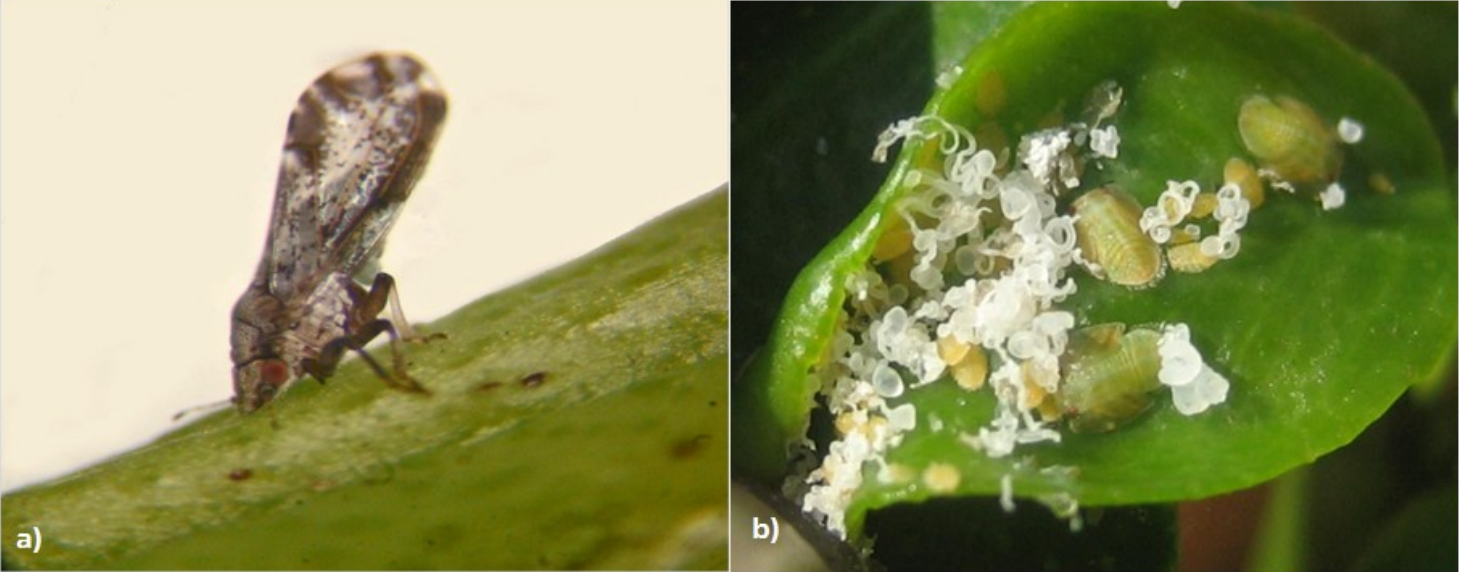
\includegraphics[width=1\textwidth,keepaspectratio=true]{images/C2/2.png}
\caption{a) Adulto, b) Ninfas de Diaphorina citri. Fotografía S. Patiño, R. Lomelí y E. Rodríguez.}
\end{figure}

Los adultos no son capaces de hacer largos viajes mediante el vuelo, de modo que su aparición a grandes distancias es debida más bien a las corrientes de aire, lo que reafirma su naturaleza sedentaria y da un mayor lapso de tiempo para que haya un contagio, tanto de la planta al psílido como del psílido a la planta. El contagio desde la planta al insecto tiene lugar normalmente cuando el psílido se encuentra en un estado ninfal, pero también puede darse cuando éste es adulto, cosa que sucede al momento de que se alimenta de la planta\cite{lopes2006vetor}.


\subsection{Formas de combate al HLB y relevancia económica}
%Control
Más adelante en este trabajo, hay un capítulo entero que aborda la metodología de control usada en México, pero a continuación se mencionan algunos de los métodos y estrategias que son usados en la industria agrícola mundial, siendo algunas de estas estrategias probadas en este trabajo. En primer lugar, se puede hablar del control por plantación de especies inhibidoras, que aunque no es uno de los métodos de control más explorados para el HLB, es de interés porque tiene una notable presencia. Este método consiste en plantar, entre los árboles cítricos, algunos árboles de Guayaba, que tienen propiedades tóxicas para el psílido, de modo que se crean barreras naturales para evitar que el psílido pase a otros árboles. Luego, en contraste con el método anterior, el control químico es de lejos el más utilizado en el campo y el más conocido debido a sus alcances. Otra práctica común es remover los árboles infectados para que éstos no hagan portadores a más psílidos y a su vez contaminen a otros árboles. Una desventaja de esta práctica es que, como se ha visto antes, algunos árboles pueden ser asintomáticos, de modo que es posible tener árboles positivos esparciendo la enfermedad dentro de cierta vecindad sin que se pueda hacer nada; esta estrategia ha sido especialmente relevante en este trabajo, pues tiene un contraste directo con el efecto asintomático.\\
También se ha de decir que existen otras alternativas biológicas de control, por ejemplo, es posible inducir parásitos a las ninfas del psílido, de modo que aumente su mortalidad y su población se vea reducida en virtud de que con esto también disminuyan los contagios de HLB. Finalmente,  es importante decir que los cultivos difícilmente están aislados del todo, esto es, que cuando un campo tiene solo árboles sanos, debería permanecer así por siempre, puesto que ninguno de sus árboles puede contagiar a otro; sin embargo, esto no sucede así en la realidad, de manera que se infiere que la infección por HLB tiene que llegar, necesariamente desde el exterior. Esto no es trivial, debido a que se ha visto que la salud de los cultivos de la región está fuertemente relacionada con la salud de cada cultivo particular\cite{robles2012protocolo}. Esto implica que controlar la infección desde dentro es inútil si el cultivo está en una zona donde hay cultivos con infecciones, puesto que se está mucho más expuesto a las amenazas del exterior, para esto se tienen en México las \textit{Áreas Regionales de Control} (ARCOs) del HLB, de las que se hablará en el siguiente capítulo.

%&Importancia económica
Según los datos en los que se han basado las Normas Oficiales Mexicanas, publicadas por el Gobierno Federal en el Diario Oficial de la Federación, que están encaminadas a combatir el Huanglongbing en México, esta bacteria ya desde 2007 representaba una amenaza para 526 mil hectáreas de cítricos, que implicaban una producción de 6.7 millones de toneladas anuales, con un valor que, ajustado a la inflación según el INEGI, hoy equivaldría a 15 mil millones de pesos, poniendo en riesgo a los 67 mil productores que entonces generaban aproximadamente 70 mil empleos directos y 250 mil indirectos.

%Cierre
Estas han sido algunas características generales del Huanglongbing que son de gran importancia para entender las motivaciones de este trabajo, los objetivos y el objeto de las decisiones tomadas al hacer las simulaciones computacionales. No se profundizará más a partir de aquí en el aspecto interno de este padecimiento, dado que la intención de este trabajo es observar la propagación desde las plantas sanas a las infectadas a través de su vector, de modo que es de poco interés, en este contexto, hablar de cuestiones como el mecanismo mediante el cual la bacteria ocasiona los síntomas de las plantas.


%-----------------------------------------------------------Qué son los sistemas dinámicos 

\section{Los sistemas dinámicos complejos}

Para partir de una base elemental, habrá que acordar qué se entiende por «sistema» y cómo su estudio da pie en ciertas instancias al uso necesario de herramientas computacionales dada su complejidad. En primer lugar, se debe decir que se entiende por \textit{sistema} a cualquier objeto, no necesariamente material, constituido por múltiples componentes que se relacionan entre sí, y evitando profundizar en motivos filosóficos, se puede entender de forma intuitiva a un sistema como \textit{un conjunto de elementos que no puede ser estudiado a través del estudio individual de estos elementos}. Esto implica que son precisamente las relaciones entre los elementos del sistema lo que le da las características emergentes que lo convierten en algo más que la simple suma de los elementos que lo conforman. Si se piensa, por ejemplo, en volúmenes de pintura rosa; la mezcla de estos volúmenes de pintura rosa será otro volumen pintura rosa y nada más. Salvo el hecho de que el volumen resultante será más grande que el anterior, no existen fenómenos que lo hagan sustancialmente distinto de los volúmenes que lo conforman. Básicamente: la mezcla de pintura rosa es más pintura rosa, vaya descubrimiento. Sin embargo, esto no es trivial, porque esto no ocurre, por ejemplo, si se presta atención a las partículas de algún material, cuya mezcla formaría algún gas o, líquido o, cualquier otro tipo de material con propiedades distintas a las de la partícula que la conforman, este hecho es nada menos que el inicio de la \textit{física molecular}, pues como se ha visto ya, entender las leyes que rigen el comportamiento de las partículas, por ejemplo, su \textit{momento}, no es suficiente para entender el fenómeno macroscópico. Finalmente se ha de decir que es interesante pensar en que un objeto que no sea un sistema, uno que en efecto sí se constituya a sí mismo, sería necesariamente un objeto \textit{autorreferencial}, aunque como se ha dicho, no es competencia de este trabajo entrar en honduras filosóficas, así que más allá de este hecho curioso y dada esta poco rigurosa definición, podemos estar firmes en la idea de que los sistemas y sus propiedades no pueden ser estudiados a través del estudio individual de sus partes, y teniendo esto en mente, podemos continuar con el estudio de los sistemas dinámicos. Los sistemas dinámicos son simplemente aquellos sistemas que cambian de estado a través del tiempo sin detenerse, de modo que pueden ser descritos en función de él. Muchos de los fenómenos cotidianos son sistemas dinámicos; como el movimiento de los cuerpos en física, el crecimiento de alguna población en biología o la evolución del PIB de alguna región en economía. También es cierto que otros ámbitos del conocimiento no se pueden abordar desde un punto que involucre al tiempo, como las leyes de un estado en derecho, la lógica formal en filosofía y hasta el equilibrio con el que cuelga un candelabro de algún teatro, siendo este último ejemplo un caso de especial interés dado que de él puede decirse que su movimiento tiende a cero conforme pasa el tiempo. Es posible sacar a este candelabro de su equilibro y hacerlo balancearse, incluso se puede estudiar su movimiento, pero finalmente siempre volverá a colgar en reposo. Decimos que este sistema tiende a un \textit{estado estacionario}, esto es, que sus variables no cambian con el tiempo.\\
Por otro lado, dentro de los sistemas dinámicos existe una parte que son los sistemas complejos, los sistemas complejos se caracterizan porque las relaciones que hay entre sus elementos añaden información extra, esto es que, a diferencia de un sistema común, no sólo no podemos entenderlos a través del estudio individual de sus elementos, sino que tampoco podemos estudiar individualmente las relaciones entre ellos, haciendo que carezca de sentido cualquier tipo de enfoque particular cuando se pretende entender un sistema como estos, de modo que las técnicas para estudiarlos tienen que ser algo más sofisticadas. Definamos vagamente a un sistema complejo como fuera definido por Herbert Simon en 1962 \cite{weaver1991science}: una red formada de elementos cuya interacción suele ser  \textit{no lineal}. Los sistemas complejos tienen la capacidad de manifestarse y cambiar mediante la \textit{autoorganización}, de una forma tal que no son absolutamente homogéneos pero tampoco son absolutamente aleatorios, y es esto lo que induce esas características emergente a nivel macroscópico de las que hemos hablado antes. Finalmente, aunque no entraremos en este terreno, es de interés decir que hay un tipo más sofisticado de sistema complejo; el sistema caótico. Un sistema caótico es un sistema dinámico complejo en el que pequeños cambios en sus variables iniciales, producen eventualmente grandes cambios en las variables finales. Esto hace que el estudio de estos sistemas no pueda ser abordado de la forma en la que se han estudiado otros en el pasado dado que cualquier sutil error de medición puede cambiar drásticamente la predicción de su comportamiento. El ejemplo típico es el del clima, se ha visto que al intentar hacer predicciones del comportamiento del tiempo en los próximos días, estas coinciden para los primeros días, pero conforme tratamos de predecir más y más días en el futuro las predicciones difieren arbitrariamente una de otra. Podríamos decir que con los modelos actuales del clima, no se puede hacer una predicción razonable sobre cómo estará el tiempo dentro de más de tres días, y esto se debe justamente a que el sistema es caótico y que pequeños cambios en las mediciones que hagamos para su predicción hacen que los resultados difieran tanto, que simplemente sería más acertado usar la estadística meteorológica.\\
Volviendo al tema que ocupa a esta sección, se ha de mencionar que las cualidades de las que gozan los sistemas mencionados anteriormente son cualidades presentes en muchos sistemas del mundo real, como los procesos fisiológicos involucrados en los organismos, las redes sociales, los fenómenos macroeconómicos, las cadenas alimenticias, los procesos neurológicos, los mercados de valores, el desarrollo del poder político y las civilizaciones, y un afortunadamente largo etcétera. Hay que puntualizar que no se debe confundir «complejo» con «complicado», existen sistemas que carecen de complicación, es decir que son simples, pero su comportamiento es complejo, y por otro lado también existen sistemas cuyo comportamiento no es complejo a pesar de ser tremendamente complicados. Además, algunos sistemas pueden ser estudiados individualmente; sistemas como dados cayendo o gases, pueden ser estudiados por la teoría de la probabilidad y física molecular respectivamente sin tener complejidad a pesar de que el fenómeno sea bastante complicado, y esto es porque se estudian sus componentes como independientes. En el otro lado, están por ejemplo los cuerpos rígidos o el lanzamiento simultáneo y combinado de dados, que tampoco son sistemas complejos, y pueden ser estudiados como sistemas acoplados. Sin embargo existe una zona en la que no hay sistemas completamente independientes o completamente acoplados, estos sistemas están en una zona que parece tener algo de organización dentro de su naturaleza compleja, esta naturaleza interdependiente puede ser abordada desde las matemáticas y la computación . Históricamente hay dos conceptos fundamentales que están involucrados en los sistemas complejos; los fenómenos emergentes y la autoorganización. En primer lugar, el concepto de los fenómenos emergentes llegó más bien de una forma filosófica, como resultado de los diversos procesos naturales en los que las propiedades del sistema a nivel macroscópico no pueden derivarse de leyes o modelos a nivel microscópico. Por ejemplo, para la medicina es trivial tener la certeza de si una persona está consciente o no, pero difícilmente podrá explicar de una forma precisa a nivel químico y físico cada uno de los procesos involucrados en la consciencia, similarmente esto sucede con las sociedades, es fácil decir qué regiones tienen un mayor índice de Desarrollo Humano o la mayor tasa de mortalidad infantil, pero difícilmente se podrá explicar exactamente qué incidentes particulares provocan estos hechos. A pesar de que en la elaboración de este texto se han encontrado varias definiciones distintas del concepto de “fenómenos emergentes”, por lo que parece no haber un consenso claro, hay algunas ideas comunes en la mayoría de estas definiciones consultadas, en primer lugar, el hecho de que los fenómenos emergentes (a veces también llamados emergencia o surgimiento) existen propiedades a escala macroscópica que son sustancialmente distintas de lo que se derivaría en principio de las leyes con las que se describe la escala macroscópica, de modo que hay emergencia de propiedades que no estaban evidentemente ahí cuando el análisis era puramente microscópico. Justamente, en este punto yace lo que le da interés a los fenómenos emergentes, que no son triviales, que hasta hoy no se conoce alguna forma simple de descubrir cómo se relacionan las propiedades de los elementos individuales del sistema que conforman. La autoorganización es también otro punto de importancia fundamental en el estudio de los sistemas complejos, que aunque pudiera parecer, no es lo mismo que las propiedades emergentes. La diferencia es que las propiedades emergentes son un asunto relacionado solamente con la escala (en tamaño), mientras que la autoorganización está relacionada además con el tiempo. De modo que se dice que algo es autoorganizado cuando al cabo de un tiempo  aparece espontáneamente un orden en el sistema en forma de alguna estructura o comportamiento regular a nivel macroscópico, y aunque parece que esto implicaría que la autoorganización es una paradoja o que contraviene la segunda ley de la termodinámica, esto no es así, desde luego, como lo veremos a continuación. A estas alturas el lector habrá pensado ya en varios sistemas cotidianos, naturales o sociales que exhiben un comportamiento de autoorganización, sin embargo habrá de estar tranquilo porque hasta ahora parece claro que ninguno de esos sistemas viola realmente la inexorable segunda ley de la termodinámica, y el secreto está en que estos son sistemas que no están ni cerrados ni aislados, tal como lo exigiría esta ley.
Para sintetizar lo anterior, los sistemas complejos son aquellos en los que surgen estructuras y comportamientos no triviales en sus propiedades macroscópicas como consecuencia de sus propiedades microscópicas, ya sea después de algún tiempo o al instante.
%Cerrar hablando de determinismo
Para terminar con esta sección, es bueno mencionar que la forma en la que se han estudiado tradicionalmente los sistemas físicos es \textit{determinista}, esto es que se tiene como un axioma la idea de que

%-----------------------------------------------------------Qué es la Simulación Computacional y el modelado

\section{La simulación computacional y el modelado matemático}
%Modelado matemático
«\textit{Ceci n'est pas une pipe}» (Esto no es una pipa), dice con grandes letras aquel cuadro surrealista de René Magritte en el que flagrantemente dibuja una pipa. Y en efecto, aquella obra del pintor francés no es una pipa sino una representación de una pipa, además de un doloroso recordatorio de que \textit{símbolo} y \textit{referente} son términos que no se deben confundir. Anteriormente no entramos en honduras filosóficas ni tampoco entraremos aquí en honduras lingüísticas, así que podemos ser simples y decir que los símbolos son los signos que usamos para evocar objetos o referentes, pero no son el objeto en sí, del mismo modo que un dibujo de una papa no es una papa. Y sí, esto es relevante para lo que sigue porque en ciencia sucede algo muy similar: toda la literatura que existe sobre los fenómenos naturales no es el fenómeno natural en sí, y más desolador aún, las imágenes mentales que se hacen los científicos de esos fenómenos tampoco son el fenómeno en sí. Es entonces osado decir que la labor del científico es la de entender la realidad, más bien esta labor se limita solamente a construir modelos cuyas predicciones sean consistentes con las observaciones experimentales en el mejor de los casos. Sin embargo, esta es seguramente la más noble de las labores humanas; la observación de la naturaleza, el modelado de sus fenómenos y la rigurosa prueba de estos modelos de forma experimental. La ciencia es modelar, y modelar es, de una forma poco rigurosa; crear una representación simple de un sistema.\newline
En cierto modo los seres humanos, para interactuar con el exterior y constituirse como tal, deben crear modelos en su mente, las tareas cognitivas cotidianas están basadas en modelos del exterior. Los modelos de la ciencia, sin embargo son más sofisticados, no son algo que surja espontáneamente en la mente, son un esfuerzo colectivo que trasciende las vidas de los científicos y son el único contacto racional que se tiene con la inclemente realidad, además de que en última instancia, todo este conjunto modelos, esta ciencia, sirven para controlar la naturaleza. Los modelos son a menudo una descripción centrada en el comportamiento de los sistemas, se enfocan en las características en puntos fijos del tiempo, ejemplos de esto son los mapas o diagramas, aunque también existe un enfoque que aborda el estudio de los sistemas desde el punto de sus reglas más que de su descripción, como las leyes de Newton, por ejemplo. Este es un enfoque dinámico que más que describir, explica el comportamiento de los sistemas, este tipo de abordaje de los problemas permite hacer predicciones sobre ellos, aunque ambas son igual de relevantes en la ciencia. Naturalmente, este trabajo tiene un enfoque que pretende explicar y predecir.\\
Claramente la labor de modelar la realidad no es sencilla, pero cuando se trata de modelar sistemas complejos, esto se suele complicar más, y esto se debe a lo hablado anteriormente, son las características propias del sistema como las propiedades emergentes, la autoorganización o los comportamientos no lineales, las que complican el modelado de estos sistemas. Para los físicos, es una herramienta confiable hacer simplificaciones y suposiciones al modelar, y esto suele ser una herramienta muy poderosa para la mayoría de sistemas típicos, por eso es común que la forma de abordar esto considere solamente cierta escala, y que si el razonamiento está dentro de una estala, se desarrolle ahí pero que nunca escale a otra, de modo que las secuencias en el proceso de pensar siguen el curso de la causalidad de una forma lineal. Y esto es algo que se ha de evitar cuando se pretenda comprender sistemas complejos, en esta instancia se debe considerar que existen muchos elementos interactuando entre sí pero independientemente, hecho que genera las ya discutidas repercusiones en otras escalas. Dicho esto, finalmente podemos deducir que los sistemas complejos son por lo común poco intuitivos y difíciles de entender, siendo esto incluso imposible a veces.\\
Pero claramente esto no puede terminar así, la conclusión no puede ser que estudiar estos sistemas es difícil y ya. Es cierto que las habilidades y la experiencia para encontrar las relaciones entre lo macroscópico y lo microscópico no son comunes a todos, pero sí es cierto que se pueden adquirir y desarrollar, y esto es tan simple como la práctica. Evidentemente es complicado acceder a las propiedades microscópicas y macroscópicas de muchos sistemas para adquirir práctica, sin embargo, las herramientas computacionales hacen que esto sea accesible y escalable. Se puede siempre construir un modelo propio al gusto con cada detalle, con cada regla y propiedad microscópica escritas en el código de la simulación para después ejecutarla y observar su comportamiento en un nivel macroscópico, que tendría que manifestar esos deseados fenómenos emergentes y de autoorganización.\\
En este trabajo seguimos ciertos criterios que han dirigido el desarrollo de la simulación, en primer lugar y como pieza clave de la ciencia, se ha buscado que el modelo pueda predecir en cierta medida razonable la realidad, sin esta característica este modelo sería de ningún interés científico además de que en la práctica tampoco tendría utilidad, si las predicciones del modelo no coincidieran o se acercaran consistentemente a los que se observa a través de la experiencia, entonces significaría que no es una representación de la realidad, que es como hemos visto antes, su único fin, de modo que su única utilidad es la de saber en qué dirección no seguir. Dado esto, se nota fácilmente la importancia de poner a prueba los modelos desarrollados y demostrar su validez; esto tanto en el ámbito de las suposiciones de las que se ha partido en su desarrollo como de las predicciones que obtenemos de él, y esto se logra a través de verificar que toda suposición sea consistente con el resto del conocimiento científico. Como probablemente el lector haya experimentado ya, es común encontrarnos con modelos de la realidad poco científicos, que a pesar de que algunos pueden rebuscados y en buena medida, libres de contradicciones, parten de bases falsas o de las que no se puede verificar la veracidad, de modo que todo el sistema carece de sentido científico, como sucede con las llamadas seudociencias.  Esto se agrava con los sistemas en los que es difícil o directamente imposible realizar alguna comparación entre la predicción que da el modelo y la evidencia de forma cuantitativa. De modo que un modelo que tenga estas características es difícil de poner a prueba y puede ser susceptible de no ser riguroso, sin embargo se ha de procurar prestar atención a los principios de los que se parte. Es en este punto donde se ha de hablar de la segunda pieza clave en este desarrollo,  buscar la simplicidad tanto como la validez. Es sensato notar que en la medida en la que se aumenta la complejidad del modelo, se suele obtener un mejor acercamiento a los datos que se observan experimentalmente, sin embargo esto puede ir en detrimento de la simplicidad, y esto hace que el modelo pierda, generalización para cuando se trata de predecir otros casos. De modo que se necesita un equilibrio para poder describir en la medida de lo posible lo general tanto como lo particular.\\
En efecto, buscar la simplicidad es algo fundamental en la construcción de un modelo, una razón es la de obtener descripciones cortas puesto que facilitan el trabajo y requieren menos recursos, pero también hay una razón más profunda, que la explicación más sencilla de las cosas se suele tomar por la más probable, y aunque no haya alguna prueba de que esto sea cierto en lo particular, suele funcionar en la mayoría de los casos. Es una práctica común inclinarse por las explicaciones más cortas siguiendo al famoso principio de la navaja de Ockham; en igualdad de condiciones, la explicación más simple suele ser la más probable. Además los modelos más simples son más fáciles de recordar y de aplicar, de modo que siempre que sea posible prescindir de algún parámetro o suposición debería hacerse, tal como se ha hecho en este modelado del HLB.
%La Simulación Computacional

La simulación que es objeto de esta tesis ha sido escrita en el lenguaje de programación Python, y se usarán las siguientes líneas  para describir sus ventajas y su importancia en el área de la simulación computacional y el modelado matemático, se hablará también de algunos grandes proyectos escritos en este lenguaje, pasando por la historia, no sólo de Python sino de la simulación computacional en general, para finalmente aterrizar en el modelado y análisis de sistemas complejos y particularmente del modelado basado en agentes individuales, que es el tipo de modelado que se usa en este trabajo. Por último, como finalidad de todo esto, haremos la obligada descripción del código de esta simulación.
Comencemos hablando de Python, un lenguaje que apareció por primera vez en febrero de 1991, hace treinta y un años, y que desde entonces ha ido cobrando relevancia hasta el gran ascenso de popularidad que ha tenido en los últimos años y que lo ha llevado a ser hoy día uno de los lenguajes de programación más populares entre la comunidad de desarrolladores de software. Python es un lenguaje orientado a objetos, de alto nivel, de \textit{tipado} fuerte y dinámico, estas características lo hacen perfecto para lo que atañe a nuestros intereses y por eso las describiremos una a una.
Es importante mencionar que Python es un lenguaje que admite múltiples paradigmas de programación, pero nosotros nos centraremos en el paradigma de la programación orientada a objetos. Que sea orientado a objetos es, sin mucho tecnicismo, que en este lenguaje podemos crear dentro del código unas entidades llamadas \textit{objetos}, que pueden ser pensados como los objetos de nuestra vida cotidiana, por ejemplo un árbol. Estos objetos, igual que los de la realidad, tienen características propias, a las que llamamos \textit{atributos}; por ejemplo su tamaño o el número de hojas para el caso del árbol, y también pueden tener \textit{funciones}, que pueden ser vistas como acciones de las que nuestro objeto forme parte y que a diferencia de los atributos que sólo son un registro de alguna característica de nuestro objeto, las funciones implican un proceso computacional, por ejemplo, el crecer o el perder todas las hojas para el caso del árbol pueden ser funciones del objeto. Esto hace que nuestro código se parezca más a la realidad y logra que programar en Python sea bastante intuitivo y que la simulación y el modelado se faciliten. Para aportar un poco más de información sobre cómo funciona intuitivamente la programación orientada a objetos, veamos un caso que ha surgido en esta simulación, en la que tenemos el ejemplo del objeto «Árbol», y del objeto «Psílido», que tiene algunos atributos como su posición que corresponde a la posición del árbol que la aloja, y si está infectada o no; además tiene la función de volar a otras posiciones y de infectar al árbol que la aloja. Estas dos últimas funciones modifican dos atributos, la primera modifica el atributo posición de el propio psílido, y el segundo modifica el atributo que nos dice si el árbol está o no infectado, desde luego que para que nuestra simulación sea de interés, el procedimiento para modificar estas variables no puede ser arbitrario y tiene que procurar comportarse como lo haría la propia naturaleza, de modo que de aquí se puede inferir que dentro de nuestras funciones de los objetos tiene que haber una buen modelado matemático basada en un conocimiento realista del fenómeno que se está describiendo, así que usando un lenguaje orientado a objetos, la labor se reduce a crear los objetos y luego plasmar en ellos las propiedades y comportamientos que se presuman como reales. Que sea de alto nivel puede ser entendido de una forma intuitiva como que su sintaxis es más abstracta, que se asemeja más al lenguaje que tenemos las personas que al lenguaje de las máquinas, encima Python tiene una gramática sencilla, puesto que prescinde de muchos símbolos engorrosos como el punto y coma al final de cada sentencia que se usa en ortos lenguajes de programación. El tipado fuerte se refiere a que el lenguaje distingue de una forma rigurosa los tipos de variables, por ejemplo, un número entero como la cantidad de psílidos de  que aloja un árbol, de un valor booleano (Verdadero o Falso) como lo puede ser si el árbol está infectado o no. A pesar de esta marcada distinción, Python tiene también un tipado dinámico, esto quiere decir que a diferencia de otros lenguajes de programación, en este no es necesario declarar al inicio del programa qué variables y de qué tipo de se usarán, haciendo que crear una variable sea más sencillo.
Por lo escrito anteriormente es claro ya que Python es una gran tecnología que goza además de una gran popularidad, pero este lenguaje es especialmente usado en la simulación de sistemas dinámicos complejos, y un ejemplo ilustre por su valor se puede encontrar en el \textit{PyCX} \cite{sayama_2013} que es un repositorio alojado en GitHub que contiene múltiples códigos de muestra sobre simulación de sistemas complejos, con un enfoque educativo y para la investigación. Este repositorio tiene como finalidad ser el punto de partida de proyectos para los estudiantes e investigadores que comiencen a incursionar en el campo del desarrollo de software para estudiar sistemas complejos, incluyendo códigos muestra de mapas iterativos, ecuaciones diferenciales tanto ordinarias como parciales, autómatas celulares, análisis de redes, redes dinámicas y modelos basados en agentes individuales también llamados «ABM», siendo estos últimos de especial interés para este trabajo.